The final selection option is a user specific application. 
The user specifies the application name and the input file containing the specific input information 
needed by the application when it is running in the backend. 
As will be discussed, the user is also required when they use an additional application not provided, 
to edit the tools registry file. Here they must include a new event application with this same name 
and the location where that application can be found relative to the tools application directory. 
If running on DesignSafe, that application must of course be built and available on the Stampeded2 supercomputer. 
NOTE that given how DesignSafe runs the applications through Agave, this applications file permissions must be 
world readable and executable (as when user running their application through DesignSafe and Agave, they are not running as themselves!)

\begin{figure}[!htbp]
  \centering {
    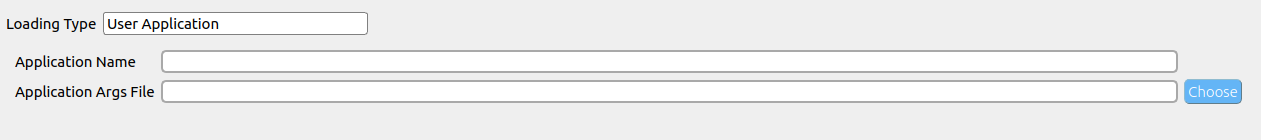
\includegraphics[width=0.8\textwidth]
    {usage/figures/userAppEvent.png} }
  \caption{User defined event}
  \label{fig:figure8}
\end{figure}
